\section{Architecture}

Abbildung \ref{fig:arch_01} zeigt einen Überblick über die Audioverarbeitungsumgebung. Der Benutzer des Systems arbeitet mit der DAW-Anwendung welches auf dem Host-CPU läuft, und kann einen Audio Plug-in auf eine bestimmte Audiospur aktivieren. Ein einzelner Audio Plug-in kann einer oder mehrere Audio Prozessoren enthalten. Prozessoren, die fähig sind ihre Aufgaben zu Verteilen suchen nach einem entsprechenden Rechenknoten auf einem Vernetztes SBC-Gerät.

Die Geräte werden über Gigabit-Ethernet vernetzt. Es wird angenommen, dass das Netzwerk nicht für sonstiges signifikanten Verkehr benützt werden.

\begin{figure}[H]
    \centering
    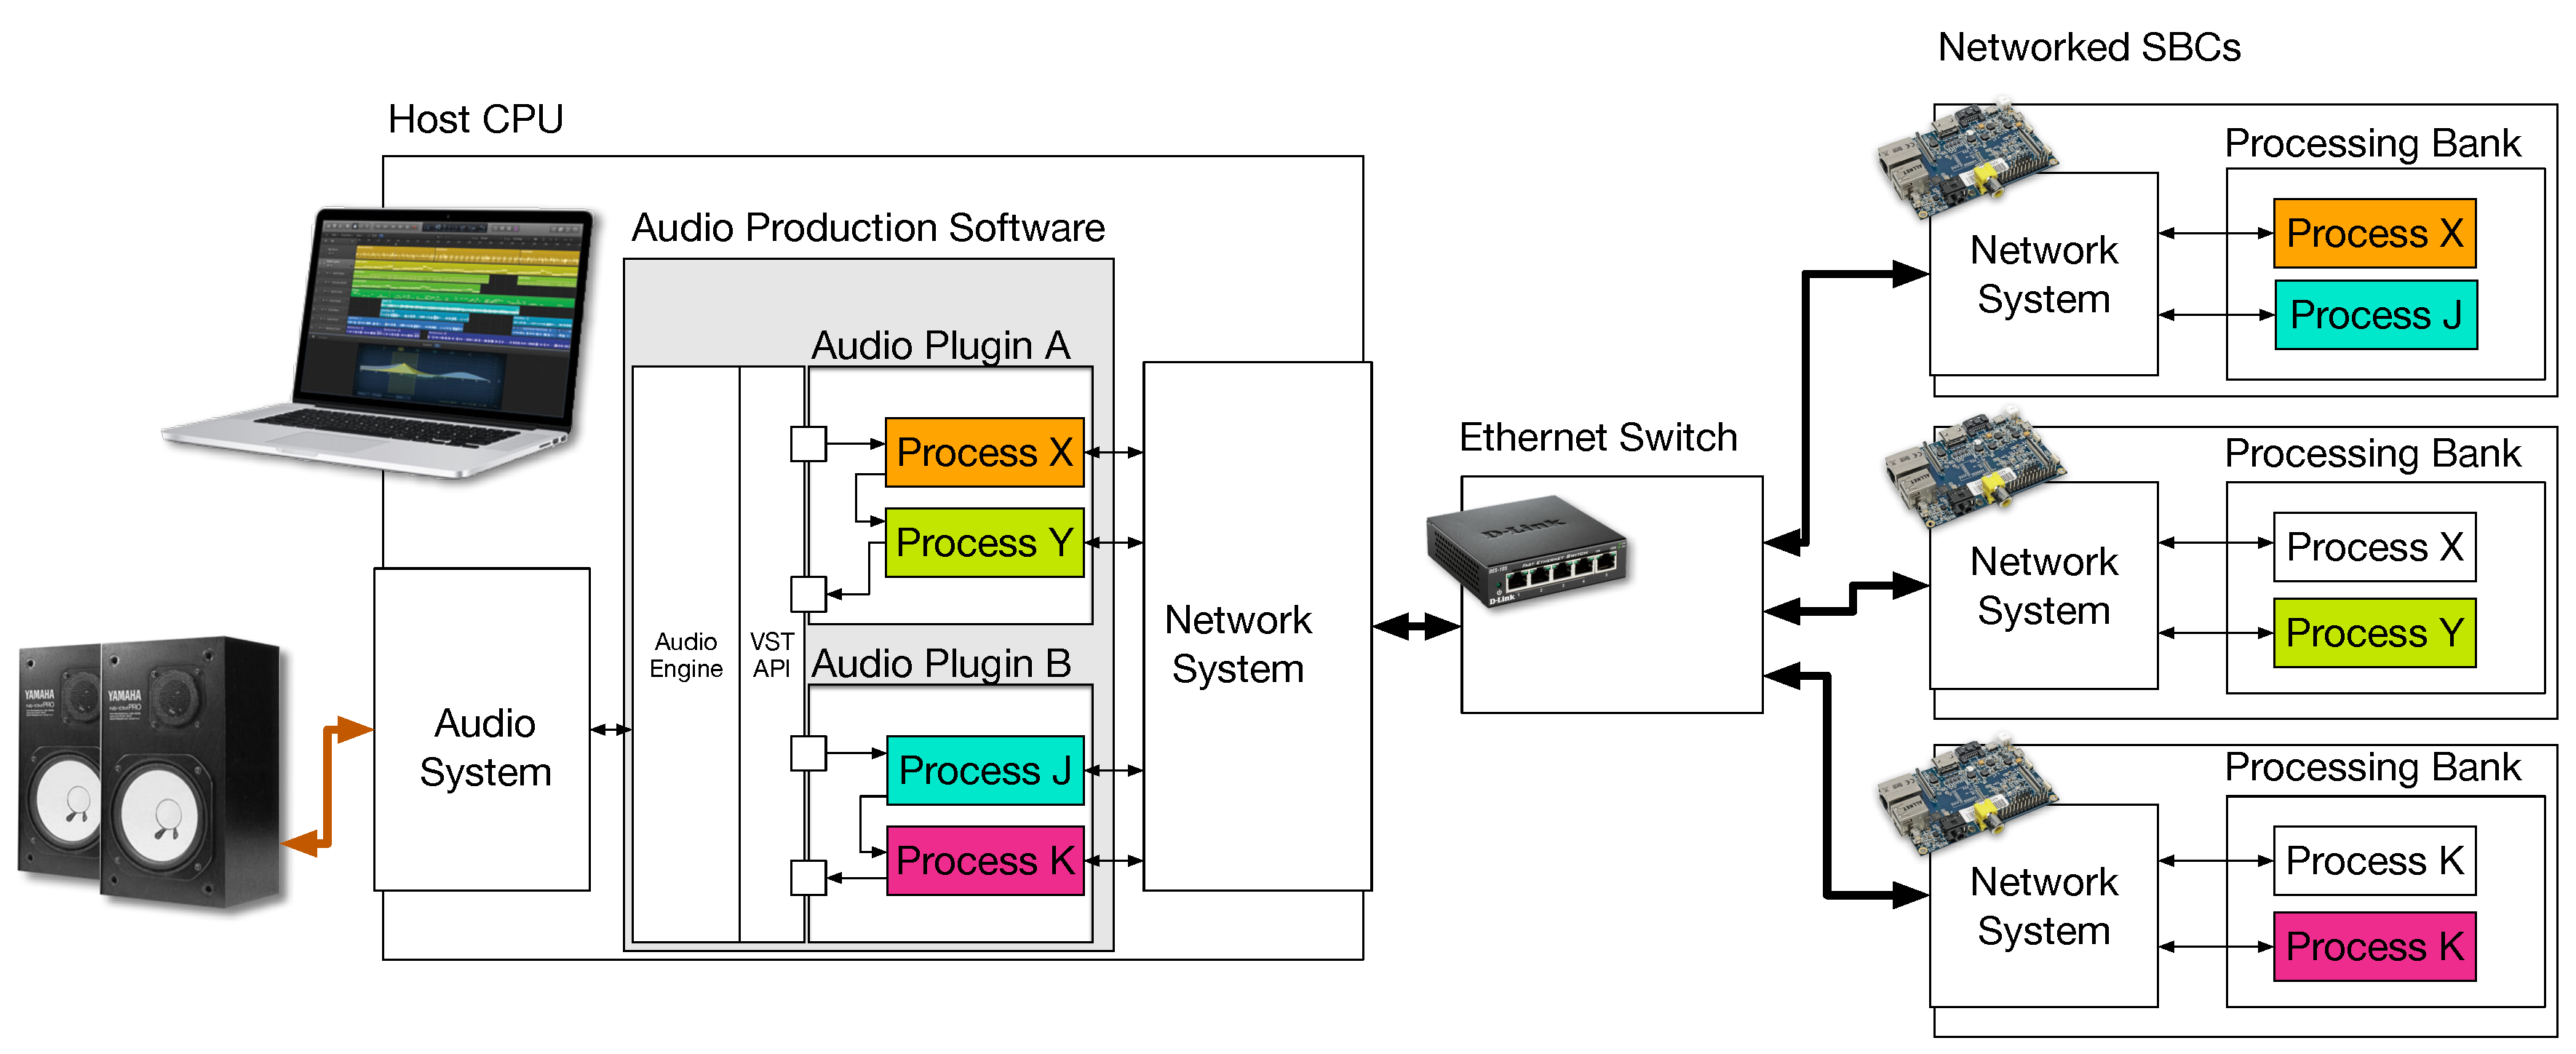
\includegraphics[width=\textwidth]{assets/architecture_01.pdf}
    \caption{Architectural Überblick}
    \label{fig:arch_01}
\end{figure}
